\section{Список смежности Iб: несколько графов}
\subsection{Условие задания}
\textbf{Вариант 8:} Построить орграф, являющийся пересечением двух заданных.

\subsection{Примеры исходного кода}
Для нахождения пересечения двух орграфов был описан метод \mitext{intersect()}:
\begin{minted}{typescript}
intersect(other: Graph): Graph {
  if (!this.oriented || !other.oriented) {
    throw new InvalidOperandTypes()
  }

  const res = new Graph(this.weighted || other.weighted, true)
  const intersection = new Map<string, Map<string, number>>()

  const commonNodes = Array.from(this.adj.keys()).filter(node => other.adj.has(node))

  for (const node of commonNodes) {
    const neighborsA = this.adj.get(node) || new Map<string, number>()
    const neighborsB = other.adj.get(node) || new Map<string, number>()
    const commonNeighbors = new Map<string, number>()

    for (const [neighbor, weightA] of neighborsA) {
      if (neighborsB.has(neighbor)) {
        const weightB = neighborsB.get(neighbor) || 0
        commonNeighbors.set(neighbor, Math.min(weightA, weightB))
      }
    }

    intersection.set(node, commonNeighbors)
  }

  res.adj = intersection
  return res
}
\end{minted}

В интерфейсе орграф"=пересечение выводится как обычно, в виде списка смежности.

\subsection{Краткое описание алгоритма}
Создается новый граф, в котором будет накапливаться результат. Затем
по определению "--- добавляем в результат только нужные вершины и дуги.

\subsection{Примеры входных и выходных данных}
\subsubsection{Входные данные}
\begin{figure}[H]
  \begin{minipage}{0.5\textwidth}
    \centering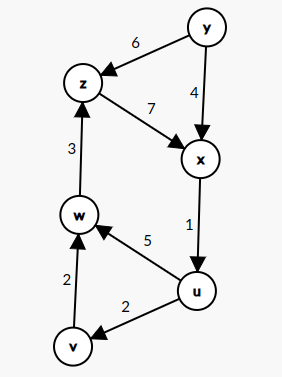
\includegraphics[width=0.6\linewidth]{figs/task-4/graph-3.png}
  \end{minipage}
  \begin{minipage}{0.5\textwidth}
    \centering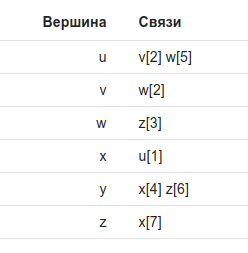
\includegraphics[width=0.6\linewidth]{figs/task-4/adj-3.png}
  \end{minipage}
  \caption{Первый ориентированный граф}
\end{figure}

\begin{figure}[H]
  \begin{minipage}{0.5\textwidth}
    \centering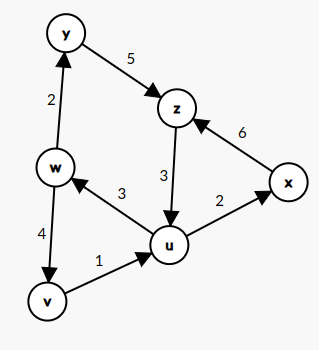
\includegraphics[width=0.6\linewidth]{figs/task-4/graph-4.png}
  \end{minipage}
  \begin{minipage}{0.5\textwidth}
    \centering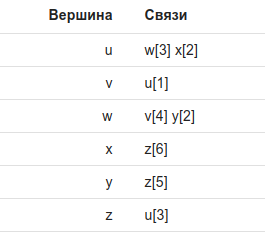
\includegraphics[width=0.6\linewidth]{figs/task-4/adj-4.png}
  \end{minipage}
  \caption{Второй ориентированный граф}
\end{figure}

\begin{minipage}{0.5\textwidth}
  \begin{minted}{js}
// первый орграф
{
  "weighted": true,
  "oriented": true,
  "adj": {
    "u": {
      "w": 3,
      "x": 2
    },
    "v": {
      "u": 1
    },
    "w": {
      "v": 4,
      "y": 2
    },
    "x": {
      "z": 6
    },
    "y": {
      "z": 5
    },
    "z": {
      "u": 3
    }
  }
}
  \end{minted}
\end{minipage}
\begin{minipage}{0.5\textwidth}
  \begin{minted}{js}
// второй орграф
{
  "weighted": true,
  "oriented": true,
  "adj": {
    "u": {
      "v": 2,
      "w": 5
    },
    "v": {
      "w": 2
    },
    "w": {
      "z": 3
    },
    "x": {
      "u": 1
    },
    "y": {
      "x": 4,
      "z": 6
    },
    "z": {
      "x": 7
    }
  }
}
  \end{minted}
\end{minipage}

\subsubsection{Выходные данные}
\begin{figure}[H]
  \begin{minipage}{0.5\textwidth}
    \centering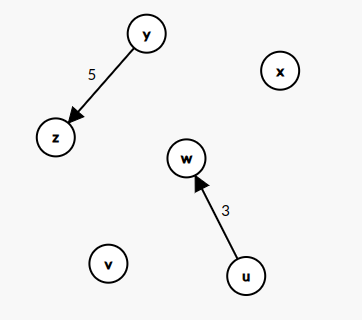
\includegraphics[width=0.8\linewidth]{figs/task-4/res-graph-4.png}
  \end{minipage}
  \begin{minipage}{0.5\textwidth}
    \centering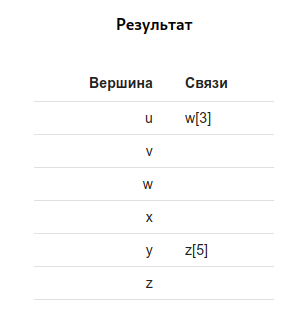
\includegraphics[width=0.8\linewidth]{figs/task-4/res-4.png}
  \end{minipage}
  \caption{Результат работы}
\end{figure}